\section{Durchführung}
\label{sec:Durchführung}

Die verwendeten Gerätschaften sind in \autoref{fig:aufbau} zu sehen.
\begin{figure}[H]
  \centering
  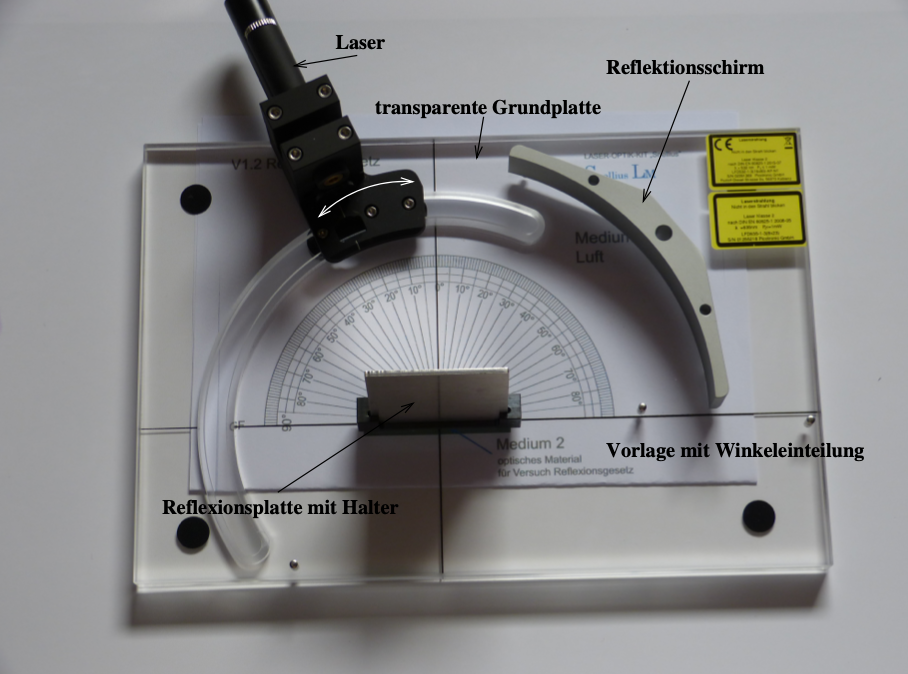
\includegraphics{content/aufbau.png}
  \caption{Die verwendete Versuchsapparatur. \cite{sample}}
  \label{fig:aufbau}
\end{figure}
An der Grundplatte sind ein roter und ein grüner Laser angebracht. 
Die Laser lassen sich auf einer Schiene im Halbkreis drehen.
Auf der Platte befindet sich im Mittelpunkt des Halbkreises eine 
Vorrichtung, auf der die optischen Elemente platziert werden.\\
Es wurden die optischen Elemente aus \autoref{fig:opt} in den verschiedenen
Versuchsteilen verwendet.\\
\begin{figure}[H]
    \centering
    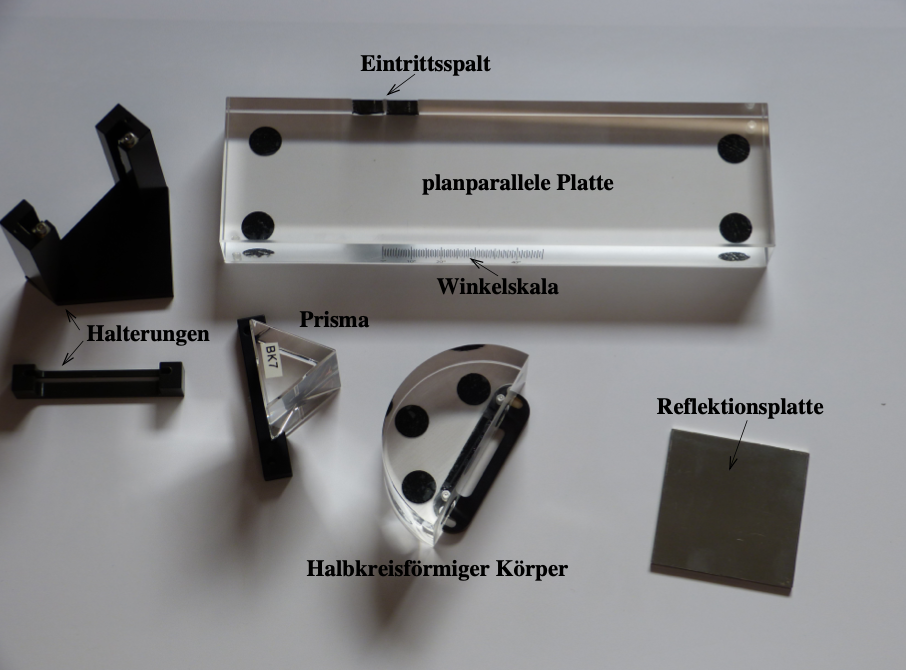
\includegraphics{content/opt.png}
    \caption{Die verwendeten optischen Elemente. \cite{sample}}
    \label{fig:opt}
  \end{figure}
Außerdem liegen verschiedene Winkelskalen vor, die unter die Grundplatte gelegt 
werden, um die Messdaten der verschiedenen optischen Elemente ablesen zu können.

\subsection*{Aufgabenteil 1}
Es wird ein Spiegel in die Vorrichtung gesetzt und mit dem grünen Laser 
7 Messwertepaare zur Verifikation von \autoref{eq:teil1} genommen.

\subsection*{Aufgabenteil 2}
Mit der planparallelen Platte werden 7 Wertepaare gemessen, mit denen \autoref{eq:teil2} 
überprüft wird. Die Platte verfügt über eine Skala, an der der 
Brechungswinkel direkt abgelesen werden kann. Es wird der grüne Laser verwendet.

\subsection*{Aufgabenteil 3}
Es wird aus den Messdaten von Aufgabenteil 2 der Strahversatz berechnet.

\subsection*{Aufgabenteil 4}
Die planparallele Platte wird durch das Prisma ersetzt. 
Mit beiden Lasern werden jeweils 5 Wertepaare für Ein- und Ausfallswinkel
genommen.

\subsection*{Aufgabenteil 5}
Mit drei Gittern der Gitterkonstanten 100, 300 und 600 werden für alle sichtbaren Intensitätsmaxima
die Winkel zum Mittelpunkt vermessen.

\section*{Vorbereitung}

\begin{table}[H]
	\centering
	\caption{Brechungsindices verschiedener Materialien. \cite{cosmos-indirekt}}
	\label{tab:brechungsindex}
	\sisetup{table-format=2.1}
	\begin{tabular}{c c}
		\toprule
		Material &
		Brechungsindex $n$ \\
		\midrule
		Luft 		& 1,000292 \\
		Wasser		& 1,33 \\
		Kronglas	& 1,46 ... 1,65 \\
		Plexiglas (PMMA) & 1,49 \\
		Diamant		& 2,42 \\
		\bottomrule
	\end{tabular}
\end{table}

Es wird in der Auswertung mit $n_{Kronglas} = 1,55$ gerechnet.
Die außerdem zu bestimmenden Gitterkonstanten lauten 
\begin{eqnarray}
    d_{100} = 10 \mathrm{\mu m} \nonumber \\
    d_{300} = 2,5 \mathrm{\mu m} \nonumber \\
    d_{600} = 1,67 \mathrm{\mu m} \nonumber 
\end{eqnarray}
